\documentclass{beamer}

\definecolor{BrickRed}{rgb}{0.8, 0.25, 0.33}

%\usetheme{CambridgeUS}%{Copenhagen}%{Frankfurt}%{Singapore}%{CambridgeUS}
\usecolortheme[named=BrickRed]{structure} 
\useoutertheme[subsection=false]{miniframes}
\useinnertheme{circles}
%\useinnertheme[shadow=false]{rounded}
\setbeamertemplate{blocks}[rounded][shadow=false]

\setbeamercovered{transparent} 
\setbeamertemplate{navigation symbols}{} %Remove navigation bar
\setbeamertemplate{footline}[frame number] % add page number
\setbeamercolor{postit}{fg=BrickRed,bg=red!10}
\setbeamercolor{structure}{bg=black!10}
%\setbeamercolor{palette primary}{use=structure,fg=red,bg=green}
%\setbeamercolor{palette secondary}{use=structure,fg=red!75!black,bg=green}
\setbeamercolor{palette tertiary}{use=structure,bg=red!50!black,fg=white}
%\setbeamercolor{palette quaternary}{fg=black,bg=green}
%\setbeamercolor{normal text}{fg=black,bg=white}
%\setbeamercolor{block title alerted}{fg=red,bg=green}
%\setbeamercolor{block title example}{bg=black!10,fg=green}
\setbeamercolor{block body}{bg= black!5}

\setbeamercolor{block title alerted}{bg=red!25}
\setbeamercolor{block body alerted}{bg=red!10}

\setbeamercolor{block title example}{bg={rgb:green,2;black,1;white,5}}
\setbeamercolor{block body example}{bg={rgb:green,2;black,1;white,20}}

\usepackage{etex} % fixes new-dimension error
\usepackage{lmodern} % fixes warnings
\usepackage{textcomp}% fixes warnings

\usepackage{graphicx,amsmath}
\usepackage{stmaryrd} % cf. interleave
%\usepackage{./macros/myisolatin1}
%\usepackage{./macros/prooftree}
\usepackage{alltt}
%\usepackage{./macros/circle}
\usepackage{listings}
\usepackage{relsize} % relative size fonts
\usepackage[normalem]{ulem} % strikethrough text (with \sout{.})
\usepackage{tikz}
\usetikzlibrary{%
  positioning
 ,patterns
 ,arrows
 ,calc
 ,shapes
 ,fit
 ,fadings
 ,decorations.pathreplacing
 ,plotmarks
% ,pgfplots.groupplots
 ,decorations.markings
}
\usepackage[normalem]{ulem} % striking out text with \sout{...}
\usepackage{xspace}

% Nicer TT fonts
\usepackage[scaled=.83]{beramono}
\usepackage[T1]{fontenc}




%------ using eurosym -------------------------------------------------------
\usepackage{eurosym}
\def\inh#1{\mbox{\small\euro}_{#1}}
\def\eith#1#2{\mathopen{[}#1 \ ,#2\mathclose{]}}

%------ using xy ------------------------------------------------------------
\usepackage[all]{xy}
%\def\larrow#1#2#3{\xymatrix{ #3 & #1 \ar[l] _-{#2} }}
\def\larrow#1#2#3{\xymatrix{ #3 & #1 \ar[l] _--{#2} }}
\def\rarrow#1#2#3{\xymatrix{ #1 \ar[r]^-{#2} & #3 }}
\def\arLaw#1#2#3#4#5{
\xymatrix{
        #1      \ar@/^1pc/[rr]^-{#4} &
        #5 &
        #2      \ar@/^1pc/[ll]^-{#3}
}}
\def\arLeq#1#2#3#4{\arLaw{#1}{#2}{#3}{#4}\leq}
%------ using pstricks (rnode etc) ------------------------------------------
%\usepackage{pstricks,pst-node,pst-text,pst-3d}
%------ using color ---------------------------------------------------------
%\newrgbcolor{goldenrod}{.80392 .60784 .11373}
%\newrgbcolor{darkgoldenrod}{.5451 .39608 .03137}
%\newrgbcolor{brown}{.15 .15 .15}
%\newrgbcolor{darkolivegreen}{.33333 .41961 .18431}
\definecolor{goldenrod}{rgb}{.80392,.60784,.11373}
\definecolor{darkgoldenrod}{rgb}{.5451,.39608,.03137}
\definecolor{brown}{rgb}{.15,.15,.15}
\definecolor{darkolivegreen}{rgb}{.33333,.41961,.18431}
\definecolor{darkgreen}{rgb}{0,0.6,0}
%
%
%\def\gold#1{{\textcolor{goldenrod}{#1}}}
\def\dgold#1{{\textcolor{darkgoldenrod}{#1}}}
%\def\brw#1{{\brown #1}}
\def\dkb#1{\textcolor{blue}{#1}}
\def\tdkb#1{\textbf{\textcolor{darkblue}{#1}}}
%%\def\gre#1{{\green #1}}
\def\gre#1{\textcolor{darkolivegreen}{#1}}
\def\gry#1{\textcolor{gray}{#1}}
\def\rdb#1{\textcolor{red}{#1}}

\definecolor{myGray}{gray}{0.85}
\newcommand{\red}[1]{\textcolor{red!80!black}{#1}\xspace}
\newcommand{\blue}[1]{\textcolor{blue}{#1}\xspace}
\newcommand{\gold}[1]{\textcolor{darkgoldenrod}{#1}\xspace}
\newcommand{\grey}[1]{\textcolor{myGray}{#1}\xspace}
\def\laplace#1#2{*\txt{\mbox{ \fcolorbox{black}{myGray}{$\begin{array}{c}\mbox{#1}\\\\#2\\\\\end{array}$} }}}
\newenvironment{bluein}{\blue}{\black\hskip -2.5pt}

%------ contexts  ---------------------------------------------------------
\newcounter{prg}
\newenvironment{prg}[1]{\refstepcounter{prg}
\noindent
\textsc{\textbf{\arabic{prg}.}} \textsc{#1} } 
{\vspace{5mm}}

\newenvironment{sprg}[1]{
\noindent
\textsc{#1} }
{\vspace{3mm}}

\newcommand\blfootnote[1]{%
  \begingroup
  \renewcommand\thefootnote{}\footnote{#1}%
  \addtocounter{footnote}{-1}%
  \endgroup
}

\newtheorem{defi}{Defini\cao}[section]
\newtheorem{defi*}{Defini\cao}
\newtheorem{lema*}{Lema}
\newenvironment{lsbcom}
      {\footnotesize  \hrule ~\\ ~\\ {\bf \sc Nota:} }
      {\hrule  ~\\ ~\\  \normalsize}
      
\newenvironment{lsbcomi}
      {\footnotesize  \hrule ~\\ ~\\ {\bf \sc Note:} }
      {\hrule  ~\\ ~\\  \normalsize}
      
\newcommand{\fimdemo}{%
\raisebox{1.7mm}{\framebox[2mm]{\rule{0mm}{0mm}}}%
\hspace{-1.55mm}%
\rule{2mm}{0.5mm}%
\hspace{-0.45mm}%
\rule{0.5mm}{2mm}%
}

\newenvironment{intf}%
     {\traco}
    {\par \nopagebreak  \traco }
\newenvironment{demo}%
     {\vspace{-5mm}\noindent {\bf Prova:}}%
    {\par \nopagebreak  \noindent \fimdemo \vspace{3mm} }
\newenvironment{demoi}%
     {\vspace{-5mm}\noindent {\bf Proof:}}%
    {\par \nopagebreak  \noindent \fimdemo \vspace{3mm} }

\long\def\CUT#1{\relax}
\def\jnowarning#1{\typeout{Warning: #1 - document page [\thepage]}}

\newenvironment{slide}[1]{\begin{frame}\frametitle{#1}}{\end{frame}}
\long\def\marginproof#1#2{
\begin{slide}{Comments}
\footnotesize Proof of #1:\\\tiny#2
\end{slide}}

\long\def\margincomment#1{
\begin{slide}{Comments}
\footnotesize #1
\end{slide}}

\long\def\marginproof#1#2{\relax}
\long\def\margincomment#1{\relax}

\def\caixa#1{\medskip
  \begin{center}
  \fbox{\begin{minipage}{0.9\textwidth}\protect{#1}\end{minipage}}
  \end{center}}
  
  \def\caixam#1{\medskip
  \begin{center}
  \fbox{\begin{minipage}{0.9\textwidth}\protect{\vspace{-5mm}#1\vspace{-5mm}}\end{minipage}}
  \end{center}}
  
   \def\caixamm#1{\medskip
  \begin{center}
  \fbox{\begin{minipage}{0.9\textwidth}\protect{\vspace{-5mm}#1}\end{minipage}}
  \end{center}}

  
  \def\caixaaa#1{\medskip
  \begin{center}
  \fbox{\begin{minipage}{0.95\textwidth}\protect{#1}\end{minipage}}
  \end{center}}

\newcommand{\caixapeq}[2][0.71]{\medskip
  \fbox{\begin{minipage}{#1\textwidth}\protect{#2}\end{minipage}}}
  
  \def\caixapeqq#1{\medskip
  \fbox{\begin{minipage}{0.85\textwidth}\protect{#1}\end{minipage}}}
  
  \def\caixamin#1{
   \begin{center}
  \fbox{\begin{minipage}{0.70\textwidth}\protect{\vspace{-5mm}#1}\end{minipage}}
  \end{center}}


\def\endprf{\begin{flushright} $\Box$ \end{flushright} \vspace{3mm}}

%------ common jno, lab  ---------------------------------------------------------
%------------
\def\wider#1{~ #1 ~}
\def\altx#1#2{\mathopen{[}#1 \ ,#2\mathclose{]}}
\def\X{\end{document}}
\def\EXIT{ \bibliographystyle{plain} \bibliography{/Users/jno/share/texinputs/jno} \end{document}}
%------------
\def\fdep#1#2#3{#1 \mathbin{\stackrel{#2}{\rightarrow\/}} #3}
\def\lift#1{\stackrel.{#1}}
\newcommand{\N}{\mathbb{N}}
\newcommand{\Z}{\mathbb{Z}}
%\def\N{I\!\!N}                             % Nat numbers
%\def\Z{Z\!\!\!Z}                           % Integers
\def\real{I\!\!R}                           % Integers

\def\name#1{\makebox[15ex][l]{\emph{#1:}} &&}
\let\kons=\underline
\def\selup#1#2#3{#3^{#1}_{#2}}
\def\plus{\mathbin{\dagger}}
\def\asor{\mathbin{|}}                    % A | B
\def\enlist#1{\mathopen{[}#1\mathclose{]}} % [a,b,...z]
\def\from{\mathbin{\leftarrow}}
\def\listdef#1#2{\enlist{ ~ #1 \asor #2 \,}} % < f(x) | x <- l>
\def\into{\mathbin{\rightarrow}}
\let\seqdef=\listdef
\def\Seq#1{{#1}^{\star}}                 % X*
\def\f{\fun F}
\def\fuc#1{\mathsf {#1}}
\def\fun#1{\mathsf {#1}}
\def\g{\fun G}
\def\ff#1{\ap\f{#1}}
\def\gg#1{\ap\g{#1}}
\def\hfilleqn#1#2{\hfill$#1\arrayin{#2}$\hfill~}
\def\enset#1{\mathopen{ \{ }#1\mathclose{ \} }} % {a,b,...z}
\newcommand{\set}[1]{\left\{ #1 \right\}} % {a,b,...z}
\def\mcond#1#2#3{#1 \rightarrow #2,#3}
\def\bang{{!}}
\def\ap#1#2{#1\,#2}
\def\pow#1{\ap{{\cal P}}{(#1)}}           \def\pow#1{{\cal P}#1} % P(X) redefined
\def\unary#1#2{\def\arg{#2}\def\omisso{}\ifx\arg\omisso{\textsf{#1}}\else\ap{\textsf{#1}}{#2}\fi}
\def\card#1{\unary{card}{#1}}             % card 
\def\ker#1{\unary{ker}{#1}}  
\def\img#1{\unary{img}{#1}}
\def\st{\dot}
\def\len#1{\unary{len}{#1}}
\def\inds#1{\unary{inds}{#1}}
\def\dom#1{\unary{$\delta$}{#1}}
\def\rng#1{\unary{$\rho$}{#1}}
\let\ran=\rng
\def\issat{\mathbin\vdash}
\def\post#1{\hbox{post-}{#1}}              % post-#1
\def\pre#1{\hbox{pre-}{#1}}                % pre-#1
\def\presat{\mathbin{\issat_{pre}}}
\def\postsat{\mathbin{\issat_{post}}}
\def\laplace#1#2{*\txt{\fbox{$\begin{array}{c}\mbox{#1}\\\\#2\\\\\end{array}$}}}
\def\PF{{\cal PF}}
\def\ler#1{{\red \em [ read: #1]}}

\def\proj#1{\pi_{#1}}
%\def\deff{\stackrel{\rm def}{=}}          % Function definition symbol
\def\deff{\, :=\, }          % Function definition symbol
\def\setdef#1#2{\mathopen{\{} #1 \asor #2 \mathclose{\}}}
\def\asor{\mathbin{|}}                    % A | B
\def\p#1{\pi_{#1}}
\def\mvdep#1#2#3{#1 \mathbin{\stackrel{\rule[-.8ex]{0pt}{0pt}#2}{\rightharpoonup\hskip-1.5ex\rightharpoonup\/}} #3}
\def\gmvdep#1#2#3#4{#1 \mathbin{\stackrel{\rule[-.8ex]{0pt}{0pt}#2}{\rightharpoonup\hskip-1.5ex\rightharpoonup_{#4}\/}} #3}
\def\sshylo#1#2{\mean{~#1,#2~}}
\def\cata#1#2{\mathopen{(\!|}#1\mathclose{|\!)}_{{\fun #2}}}
\def\split#1#2{\const{#1,#2}}
\def\tuple#1{\mathopen{\langle}#1\mathclose{\rangle}} % <a,b,...z>
\def\divides{\mathbin{\setminus}}
\def\rdiv{\mathbin{\setminus}}
\def\ldiv{\mathbin{/}}
\def\true{\mathsf{true}}
\def\mean#1{\mathopen{[\![}#1\mathclose{]\!]}}
\def\false{\mathsf{false}}
\newenvironment{lcbr}{\left\{\begin{array}{l}}{\end{array}\right.}
\def\rcb#1#2#3#4{\def\nothing{}\def\range{#3}\mathopen{\langle}#1 \ #2 \ \ifx\range\nothing::\else: \ #3 :\fi \ #4\mathclose{\rangle}}

\def\rcbVdm#1#2#3#4{#1 \ #2 \ � #4}
\def\deffVdm{\mathbin{\raisebox{.2em}{\tiny \ \underline{$\mathchar"3234$} \ }}}
\def\mapVdm#1#2{#1 \mathbin{\tilde{\rightarrow}} #2}

\def\const#1{\mathopen{\langle}#1\mathclose{\rangle}} % <a,b,...z>
\def\comp{\mathbin{\cdot}}
\def\implied{\mathbin\Leftarrow}
\def\implies{\mathbin{\Rightarrow}}
\def\arrayin#1{\begin{array}{rcl}#1\end{array}}
\def\xarrayin#1{\begin{array}{cccccc}#1\end{array}}
\def\aspas#1{``#1''}
\def\ap#1#2{#1\,#2}
\def\unary#1#2{\def\arg{#2}\def\omisso{}\ifx\arg\omisso{\textsf{#1}}\else\ap{\textsf{#1}}{#2}\fi}
\def\card#1{\unary{card}{#1}}             % card x
\def\ker#1{\unary{ker}{#1}}  
\def\img#1{\unary{img}{#1}}
\def\ijust#1#2{&#1& \rule{2em}{0pt}  \{ \mbox{\rule[-.5em]{0pt}{1.2em} \footnotesize #2 \/} \}  \nonumber\\ && }
\def\just#1#2{\\\ijust{#1}{#2}}

\def\crflx#1{\Phi_{#1}}
\def\qcomp{\mathbin\bullet}
\def\xlarrow#1#2#3{\larrow{#3}{#2}{#1}} 
%\def\equiv{\Leftrightarrow}
\def\longlarrow#1#2#3{\xymatrix{ #3 && #1 \ar[ll] _-{#2} }}
%------------

%------  lsb  ---------------------------------------------------------

\def\drawit{\nccurve[angleA=-30,angleB=-150]{->}{NA}{NB}}

\def\cnext#1{\Circle_{#1}}
\def\clast#1{\Circle[f]_{#1}}
\def\calfut#1{\square_{#1}}

\def\mdepth#1{\mathsf{md}\, #1}

\def\always{\boxempty}
\def\eventual{\Diamond}
\def\nexts{\bigcirc}
\def\until{\mathbin{\mathcal U}}


\def\setFontSize#1{\gdef\currentFontSize{#1}\fontfamily{phv}\fontsize\currentFontSize\currentFontSize\selectfont}
\def\greybox#1{*\txt{\mbox{\fcolorbox{black}{myGray}{\mbox(40,15){#1}}}}}
\def\funbox#1{*\txt{\fcolorbox{white}{myGray}{\makebox(40,15){\black $#1$}}}}
\def\condition#1{*\txt{\fontfamily{phv}\fontsize\currentFontSize\currentFontSize\selectfont\pscirclebox[linecolor=white]{$#1$}}}
\def\checkpoint{*\txt{\pscirclebox*{}}}
\def\state{*\txt{\ovalnode[fillstyle=solid,fillcolor=red]{State}{\black Internal state}}}
\def\thing#1{$\bullet$ \rule{0pt}{.7cm} & \fcolorbox{black}{myGray}{#1}}

\def\const#1{\mathopen{\langle}#1\mathclose{\rangle}} % <a,b,...z>
\def\funbox#1{*\txt{\fcolorbox{white}{gray}{\makebox(40,15){\black $#1$}}}}
\def\pair#1{\const{#1}}
\def\bim{\fuc{B}}
%\def\abim#1{\bim\, #1}
\def\abim#1{\aapf{\bim}{#1}}
\def\bimm#1{\bim #1}
\def\iso{\cong}
\def\niso{\ncong}
\def\qcom{\mathbin{\boldsymbol{;}}}
\def\id{\fuc{id}}

\def\ainv#1{\overline{#1}}

\def\rsrt{\tau_{r}}   % right and left strength
\def\rsrtp#1{\tau_{r_{#1}}}   % right and left strength
\def\lsrt{\tau_{l}}

\def\igual{\mathbin{=}}
\def\dimp{\mathbin{\Leftrightarrow}}
\def\imp{\mathbin{\Rightarrow}}
\def\dimpp{\mathbin{\leftrightarrow}}
\def\impp{\mathbin{\rightarrow}}
\def\rimp{\mathbin{\Leftarrow}}
\def\limp{\mathbin{\multimap}}

\newcommand{\sse}{\mathbin{\, \operatorname{\textsf{iff}} \,}}
\def\e{\mathbin{\wedge}}
\def\ou{\mathbin{\vee}}

\def\aconv#1{#1^{\circ}} 
\newcommand{\fdec}[3]{#1: #2 \longrightarrow  #3}
\newcommand{\fdecf}[3]{#1: #2 \longrightarrow #3}
\newcommand{\fdef}[2]{#1\;=\; #2}

\newcommand{\adec}[3]{#1 \stackrel{#2}\longrightarrow #3}
\newcommand{\fblockf}[5]{
\begin{eqnarray*}
#1&\! \! \!: \!\! \!& #2 \longrightarrow #3\\
#1 & \! \!\! #4\, = \!\!\!& #5
\end{eqnarray*}
}

\newcommand{\sos}[3]{#3 \stackrel{#2}{\longleftarrow} #1}
\def\setcat{{\sf Set}}
\def\relcat{{\sf Rel}}
\def\parcat{{\sf Par}}
\def\predcat{{\sf Pred}}
\def\ordcat{{\sf Ord}}

\def\dois{\ensuremath{\boldsymbol{2}}}
\def\abv{\stackrel{\rm abv}{=}}
\def\sana#1{\mathopen{[\!(}#1\mathclose{)\!]}}
\def\deff{\triangleq} 
\def\pint{\mathbin{\interleave}}



% Fev 2010

\def\oculos{\mathbf{\bigcirc\!\! \frown\!\! \bigcirc}}
\def\ferramentas{\stackrel{\mathbf{\doublecap}}{\bigbox\!\!\bigbox}}
%\def\Act{\cal{N}}
\def\Act{N}

\def\vec#1{\Tilde{#1}}
\def\free#1{\textsf{free}(#1)}
\def\subs#1#2#3{\enset{#1/#2}\, #3}

\def\tim{\fuc{T}}
\def\att{\fuc{at}}
\def\md{\fuc{m}}

\def\bh#1#2{\apf{\ana{#1}}{#2}}

\def\apf#1#2{#1\; #2}                   % func applic no () -- f a
\def\appf#1#2{(#1\; #2)}                   % func applic with () -- (f a)
\def\aapf#1#2{#1 #2}                   % func applic no () -- f a

\def\aappf#1#2{(#1 #2)}                   % func applic with () -- (f a)
\def\appff#1#2{#1 (#2)}                   % func applic with () -- f(a)
%\def\ana#1#2{\mathopen{[\!(}#1\mathclose{)\!]}_{#2}}
%\def\ana#1#2{\mathopen{[\!(}#1\mathclose{)\!]}_{\fun #2}}
\def\ana#1{\mathopen{[\!(}#1\mathclose{)\!]}}
\def\sana#1{\mathopen{[\!(}#1\mathclose{)\!]}}

\def\iid#1{\id_{#1}}                     %  identitade default
\def\id{\mathbin{\fuc{id}}}    

\def\atim#1{\aapf{\tim}{#1}}
\def\final#1{\omega_{#1}}
\def\initial#1{\alpha_{#1}}

\def\ialg#1{\mu_{#1}}
\def\fcoalg#1{\nu_{#1}}
\def\hdd{\fun{hd}}
\def\tll{\fun{tl}}
\def\mrg{\fun{merge}}
\def\gnn{\fun{rep}}
\def\diag{\vartriangle}
\def\codiag{\triangledown}
\def\twist{\fun{twist}}
\def\swap{\fuc{s}}
\def\rtran#1{\stackrel{#1}{\longrightarrow}}
\def\tran#1{\stackrel{#1}{\longrightarrow}}
\def\primertran#1{\stackrel{#1}{\longrightarrow'}}
\def\rra{\longrightarrow}
\def\ppow{\ensuremath{\mathcal{P}}} 
\def\nx{\fun{next}}
\def\utran#1{\stackrel{#1}{\longrightarrow}}  % - a - > 
\def\reach#1{\stackrel{#1}{\longrightarrow}^*}

\newcommand{\blk}[1]{\mathbb{#1}}
\newcommand{\ger}[1]{\mathfrak{#1}}

\def\vs{\emph{vs}}
\def\ie{\emph{i.e.}}
\def\cf{\emph{cf.}}

\def\eg{\emph{e.g.}}

\def\PP{\blk{P}}

%------ CCS          -----------------------------------------%
\def\ppe{\mathbin{\vartriangleright}}
\def\kcomp{\mathbin{\boldsymbol{\bullet}}}
%\def\qcomp{\mathbin{\boldsymbol{;}}}
\def\ssp{\textsc{skip}}
\def\fim{\dagger}
%\def\ppe{\gg}
\def\cnil{\mathbf{0}}
\def\cpf#1#2{#1 . #2}                           % a.P
\def\cou#1#2{#1 \mathbin{+} #2}                 % P + Q
%\def\crt#1#2{\mathbin{#1 \setminus_{#2}}}       % P \ A
%\def\crtt#1#2{\mathbin{#1 \setminus\!\setminus_{#2}}}       % P \ A
%\def\crt#1#2{\mathsf{new}\, #2\;  #1}       % P \ A
\def\crt#1#2{#1 \backslash #2}       % P \ A
%\def\crn#1#2{\{#2\}\, #1}                  % P[f]

\def\crn#1#2{\mathbin{#1[#2]}}                  % P[f]
\def\couit#1#2{\Sigma_{#1}#2}                  %  + i=1,n
\def\cpar#1#2{#1 \mid #2}                       %  |
\def\ctpar#1#2{#1 \parallel #2}                       %  |
\def\cpars#1#2#3{#1 \mid_{#3} #2}               %  |S
\def\ffix#1#2{\underline{fix}~(#1\, =\, #2)}  % fix X
\def\fffix#1#2#3{\underline{fix}_{#1}~(#2\, =\, #3)}  % fix X
\def\tfix#1#2{\underline{\Tilde{fix}}~(\Tilde{#1}\, =\, \Tilde{#2})}  % fix X
%\def\ainv#1{\Bar{#1}}                   % ~ a
\def\ainv#1{\overline{#1}}                   % ~ a
\def\cif#1#2{\fuc{if}\, #1\, \fuc{then}\, #2}
\def\ccif#1#2#3{\fuc{if}\, #1\, \fuc{then}\, #2\, \fuc{else}\, #3}

\def\fres#1#2{#1 \restriction #2}                

\def\mean#1{\mathopen{[\![}#1\mathclose{]\!]}}
\def\llbracket{\mathopen{[\![}}
\def\rrbracket{\mathopen{]\!]}}

\def\cfree#1{\fuc{fn} (#1)}
\def\cbound#1{\fuc{bn} (#1)}
\def\anew#1{\overline{#1}\mathsf{new}\, } 
\def\transitatau{\rtran{\tau}}
\def\transitaa{\rtran{a}}


\def\cHat#1{{\cal T}(#1)}
\def\free#1{\textsf{free}(#1)}
\def\fuc#1{\textsf{#1}}
\def\subs#1#2#3{\enset{#1/#2}\, #3}
\def\PP{\blk{P}}
\def\PPf{\blk{P}_{\fim}}
\def\obs{\mathbin{\sim}}                     % P ~ Q
\def\nobs{\mathbin{\nsim}}                     % P ~ Q
\def\aobs{\mathbin{\approx}}                 % P ~ Q
\def\naobs{\mathbin{\not \approx}}                 % P ~ Q
\def\cobs{=}                                 % P = Q
\def\ssort#1{\blk{L}(#1)}                   % L()
\def\sysort#1{\blk{L}_s(#1)}                   % L()

\def\athen{\comp}
\def\PP{\blk{P}}

% 2015

\def\st{\mathbf{.}\,}
\def\laplace#1#2{*\txt{\mbox{ \fcolorbox{black}{myGray}{$\begin{array}{c}\mbox{#1}\\\\#2\\\\\end{array}$} }}}
\newcommand{\galois}[2]{#1\; \dashv\; #2}

\newcommand{\fddec}[3]{#1: #2 \longrightarrow  #3}

\def\mcrl{\textsf{mCRL2}}

\def\obs{\sim}
\def\eqm{\mathbin{\equiv}}                     
\def\noeqm{\mathbin{\not\!\equiv}}  
\newcommand{\flam}[2]{\lambda_{#1}\; .\; #2}
\def\existential#1#2{\exists_{#1}\;.\; #2}
\def\existencial#1#2{\exists_{#1}\;.\; #2}

\def\pv#1#2{\langle #1 \rangle\, #2}
\def\nc#1#2{[#1]\, #2}
\def\pvo#1#2{\langle \! \! \! \langle #1 \rangle \! \! \! \rangle\, #2}
\def\nco#1#2{\llbracket #1 \rrbracket #2}
\def\cvg#1{\llbracket \downarrow \rrbracket #1}
\def\cvgr#1#2{\llbracket #1 \downarrow \rrbracket #2}
\def\cvgl#1#2{\llbracket \downarrow  #1 \rrbracket #2}
\def\cvglr#1#2{\llbracket \downarrow  #1 \downarrow \rrbracket #2}
\def\lfp#1#2{\mu {#1}\, .\, {#2}}
\def\lpf#1#2{\mu {#1}\, .\, {#2}}
\def\gfp#1#2{\nu {#1}\, .\, {#2}}
\def\gpf#1#2{\nu {#1}\, .\, {#2}}
\def\mset#1{\vvv #1 \vvv}
\def\vvv{\vert \! \vert}
\def\mnc#1{\vvv [#1] \vvv}
\def\mpv#1{\vvv \langle #1 \rangle \vvv}
\def\bcomp#1{#1^{\text{c}}}
\def\eqm{\mathbin{\simeq}}
\def\noeqm{\mathbin{\not\!\simeq}}
\def\universal#1#2{\forall_{#1}\; .\; #2}
\def\existential#1#2{\exists_{#1}\; .\; #2}
\def\oexistential#1#2{\exists^{1}_{#1}\; .\; #2}

\def\reach#1{\stackrel{#1}{\longrightarrow}^*}


\def\rra{\longrightarrow}

\def\Lg#1{\mathsf{Lang}(#1)}
\def\Tr#1{\mathsf{Tr}(#1)}

\def\PP{\blk{P}}

\def\paths#1{\mathsf{Paths}(#1)}
\def\Mcomma{\text{ ,}}
\def\Msemicolon{\text{ ;}}
\def\Mdot{\text{ .}}


%%%%%%%%%%%%%%%% NUNO reconf

\def\reo{\textsf{Reo}\xspace}
\def\reolang{\textsf{CooPLa}\xspace}
\def\recoopla{\textsf{ReCooPLa}\xspace}
\def\CP{coordination pattern\xspace}
\def\CPs{coordination patterns\xspace}
\def\node#1{\ensuremath{\underline{#1}}}
\def\nameset{\ensuremath{\mathcal{I}}\xspace}
\def\endnameset{\ensuremath{\mathcal{E}}\xspace}
\def\nodeset{\ensuremath{\mathcal{N}}\xspace}
\def\portset{\ensuremath{\Sigma}\xspace}
\def\coordpatset{\ensuremath{\mathcal{P}}\xspace}
\def\logicmodel{\ensuremath{\mathcal{M}}\xspace}
\def\reconfset{\ensuremath{\mathcal{R}}\xspace}
\def\reconfoperationset{\ensuremath{\mathcal{O}}\xspace}
\def\channelset{\ensuremath{\mathcal{C}}\xspace}
\def\stateset{\ensuremath{\mathcal{S}}\xspace}
\def\typeset{\ensuremath{\mathcal{T}}\xspace}
\newcommand{\chanodesof}[2][\rho]{\ensuremath{\mathfrak{N}_{#1}^{#2}}\xspace}
\newcommand{\reconfop}{\ensuremath{\mathbin{\bullet}}}

\newcommand{\byreconfof}[1]{\ensuremath \stackrel{\rm #1}{\longleftarrow}}

\def\trans#1{\stackrel{#1}{\longrightarrow}}
\def\TS#1{\mathcal{G}(#1)}
\def\TSn#1{\mathcal{G}_{nodes}(#1)}


%%%%%%%%%%%%%%%%%%%%%%%%% ALEXANDRE
 \def\HHL{\mathcal{HHL}}
 
 \def\emskip{\vskip 1em}
 
 %%%%%%%%%%%%%%%%%%%%%% COMPONENTES NOV 2015
 \def\para{\mathbin{\boxtimes}}   % Mealy produto (sincrono)
\def\parc{\mathbin{\boxplus}}    % Mealy soma
\def\pars{\mathbin{\boxast}}     % Mealy misto
\def\shk#1#2{\bigl(#1\bigr)_{#2}}            % separated hook direita
\def\hk#1#2{#1\! \Lsh_{#2}}            % hook direita
\def\hkespaco#1#2{#1 \Lsh_{#2}}            % hook direita
%\def\feed#1{\Bigl( #1 \Bigr)\! \Lsh}            % hook direita
\def\feed#1{#1 \Lsh}            % hook direita
\def\kh#1#2{~_{#2}(#1)}           % hook esquerda

\def\flift#1{\ulcorner #1 \urcorner}           % funcoes embb
\def\singr#1{\lfloor #1 \rceil}

\def\pdiag{\bigtriangleup}      % diagonal em componentes
\def\pcodiag{\bigtriangledown}    % codiagonal em componentes

%\qcomp{\mathbin{\mathbf{;}}}
%\def\qcom#1#2{#1\qcomp#2}
%\def\sync{}  %d� problemas com o reotex.sty do Nuno Oliveria

 
 %%%%
 \def\SING{\ensuremath{\boldsymbol{1}}}
\def\ZERO{\ensuremath{\boldsymbol{0}}}

\def\ptran#1{\stackrel{#1}{\leadsto}}
\def\pptran#1#2{\stackrel{#1[#2]}{\leadsto}}

\def\bblue#1{\dkb{#1}}
\def\ctt#1{\underline{#1}}    
\def\lvazio{\fuc{nil}}   
\def\lcons{\mathbin{\fuc{cons}}} 
\def\either#1#2{[#1,#2]}
\def\att{\fun{at}}
\def\hd#1{\mathbin{\fuc{hd}} \, {#1}}              % hd x
\def\tl#1{\mathbin{\fuc{tl}} \, {#1}}   
\def\hdd{\mathbin{\fuc{hd}}}              % hd x
\def\tll{\mathbin{\fuc{tl}}}              % hd x\def\nnat{\blk{N}}
\def\rreal{\blk{R}}
\def\nnat{\blk{N}}
\def\vtran#1#2#3{#1\downarrow_{#3} #2 }
\def\labtran#1#2{~_{#1}\!\stackrel{#2}{\longleftarrow\, }}
\def\rabtran#1#2{\stackrel{#2}{\longrightarrow}_{#1}\, }
\def\excp#1{#1 + \SING}
\def\usplit#1#2{\langle #1, #2 \rangle}
\def\nnx{\fun{nx}}
\def\nxc{\ainv{\fun{nx}}}
%\def\ct{\fun{ct}}
%\def\ctc{\ainv{\fun{ct}}}
%\def\ini{\fun{ini}}
\def\nil{\underline{\fun{nil}}}
\def\att{\fun{at}}
\def\nx{\fun{next}}
\def\md{\fun{m}}
\def\acc{\ainv{\fun{ac}}}
\def\ac{\fun{ac}}
\newcommand{\mcar}[3]{(#1\, \rightarrow\, #2, \,   #3)}
\def\distr{\fuc{dr}}
\def\distl{\fuc{dl}}
\def\hdi#1{\mathbin{\fuc{last}} \, {#1}}              % hd x
\def\tli#1{\mathbin{\fuc{blast}} \, {#1}} 
\def\ip#1{\iota_{#1}}
\def\apf#1#2{#1\; #2}   
\def\m{\fuc{M}}

\def\onefuc{\fuc{Id}}
\def\triple#1{\const{#1}}
\def\kcomp{\mathbin{\boldsymbol{\bullet}}}  
 
\def\ntarrow{\Longrightarrow}
\newcommand{\ntdec}[3]{#1: #2 \ntarrow #3}
\def\ntiso{\stackrel{\iso}{\ntarrow}}

\def\rsrt{\tau_{r}}   % right and left strength
\def\rsrtp#1{\tau_{r_{#1}}}   % right and left strength
\def\lsrt{\tau_{l}}
\def\lsrtp#1{\tau_{l_{#1}}}   % right and left strength
\def\deltab{\delta}
\def\rpd{\delta_{r}}   % strength combination
\def\rpdp#1{\delta{r_{#1}}}
\def\lpd{\delta_{l}}
\def\ltrocam{\fuc{xl}_{+}}  % \assoc inv . \swap . \assoc
\def\rtrocam{\fuc{xr}_{+}}  
\def\dtrocam{\fuc{m}_{+}}  
\def\ltroca{\fuc{xl}}  % \assoc inv . \swap . \assoc
\def\rtroca{\fuc{xr}}  
\def\dtroca{\fuc{m}}  
\def\troca{\fuc{x}}  
\def\cat#1{{\sf #1}}
\def\flift#1{\ulcorner #1 \urcorner} 
\def\PR{\cat{Cp}}
\def\PRSp{\cat{Cp}_{Sp}}
\def\prcat#1{{\sf Cp_{#1}}}
%\newcommand{\prhom}[2]{\PR_{\bim}(#1, #2)}
\newcommand{\prhom}[2]{\PR(#1, #2)}
%\newcommand{\prhoms}[2]{\PR_{\bim}(#1, #2)_{Sp}}
\newcommand{\prhoms}[2]{\PR(#1, #2)_{Sp}}
\def\cid#1{\fuc{copy}_{#1}} 
\def\bismp#1{\sim{#1}}
\def\bism{\mathbin{\sim}}
\def\nbism{\overset{\bullet}{\sim}}
\def\nobism{\mathbin{\not\!\sim}}
\def\nilc{\fuc{nil}}
\def\idle{\fuc{idle}}
\def\inert#1{\fuc{inert}_{#1}}
\def\zerol{\fuc{zl}}
\def\zeror{\fuc{zr}}
\def\distr{\fuc{dr}}
\def\distl{\fuc{dl}}
\def\assoc{\fuc{a}}
\def\assocs{\fuc{a_*}}
\def\assocm{\fuc{a_+}}
\def\swap{\fuc{s}}
\def\swaps{\fuc{s_*}}
\def\swapm{\fuc{s_+}}
\def\lunit{\fuc{l}}
\def\runit{\fuc{r}}
\def\lunits{\fuc{l_*}}
\def\runits{\fuc{r_*}}
\def\lunitm{\fuc{l_+}}
\def\runitm{\fuc{r_+}}
\def\ana#1#2{\mathopen{[\!(}#1\mathclose{)\!]}_{#2}}
\def\sana#1{\mathopen{[\!(}#1\mathclose{)\!]}}
\def\bh#1#2{\apf{\ana{#1}}{#2}}
\def\BH{\cat{Bh}}
\def\diag{\vartriangle}
\def\codiag{\triangledown}
\def\psplit#1#2{\mathopen{\langle}#1, #2\mathclose{\rangle}}
\def\flift#1{\ulcorner #1 \urcorner} 
\def\rpdp#1{\delta{r_{#1}}}
\def\lpd{\delta_{l}}
%\def\lpdp#1{\lpd_{#1}}
\def\lpdp#1{\delta{l_{#1}}}

\def\bunit#1{\eta_{#1}}   % monad unit
\def\bmul#1{\mu_{#1}}   % monad multi

\def\bag#1{\fuc{Bag}_{#1}}

\newcommand{\MH}{\mathcal{H}}
\newcommand{\M}{M}
\newcommand{\Rz}{\textsc{T}}
\newcommand{\docircrlh}[2]{%
  \ooalign{$#1\rightarrow$\cr\hfil$#1\comp$\hfil\cr}}
\newcommand{\karrow}{\mathrel{\mathpalette\docircrlh\relax}}
\newcommand{\eqdef}{\widehat{=} \> \>}
\newcommand{\conc}{\> {\small \texttt{+} \hspace{-0.1cm} \texttt{+}} \>}
\newcommand{\mtime}{ [ 0, \infty ) }
\newcommand{\longerarrow}{\xrightarrow{\hspace*{1cm}}}
\newcommand{\klH}{\topo_{\MH}}
\newcommand{\topo}{{\bf Top}}
\def\hmul#1#2#3 { #1 \> \lhd \> #2 \> \rhd \> #3 }
\def\qcompp{\mathbin{\boldsymbol{;}}}
\def\qcom#1#2{#1\qcompp#2}


%--------------------
%--- by jose 2016 ---
%--------------------

\newcommand{\wrap}[2][]{\begin{tabular}[#1]{@{}c@{}}#2\end{tabular}}
\newcommand{\mwrap}[1]{\ensuremath{\begin{array}{@{}c@{}}#1\end{array}}}
\newcommand{\myblock}[1]{\begin{beamercolorbox}[dp=1ex,center,rounded=true]%
  {postit} {\large \textbf{#1}} \end{beamercolorbox}}%
\def\trans#1{\xrightarrow{#1}}  % - a - > 
\def\Trans#1{\stackrel{#1}{\Longrightarrow}} % =a=> 
\newcommand{\transp}[2][35]{\color{fg!#1}#2}
\newcommand{\transpt}[2][.35]{\tikz{\node[inner sep=1pt,fill opacity=0.5]{#2}}}

\newcommand{\frsplit}[3][.48]{
  \begin{columns}%[T] % align columns
  \begin{column}{#1\textwidth} #2 \end{column} ~~~
  \begin{column}{#1\textwidth} #3 \end{column} \end{columns}
}
\newcommand{\frsplitt}[3][.48]{
  \begin{columns}[T] % align columns
  \begin{column}{#1\textwidth} #2 \end{column} ~~~
  \begin{column}{#1\textwidth} #3 \end{column} \end{columns}
}
% rules
\newcommand{\typerule}[4][]{\ensuremath{\begin{array}[#1]{c}\textsf{\scriptsize ({#2})} \\#3 \\\hline\raisebox{-3pt}{\ensuremath{#4}}\end{array}}}
\newcommand{\styperule}[3][]{\ensuremath{\begin{array}[#1]{c} #2 \\[0.5mm]\hline\raisebox{-4pt}{\ensuremath{#3}}\end{array}}}
\newcommand{\shrk}{\vspace{-3mm}}


\newcommand{\evm}[1]{\langle #1 \rangle\,}
\newcommand{\alm}[1]{[#1]\,}

\newcommand{\myparagraph}[1]{\medskip\noindent\textbf{#1}~~}



% Listing
\lstset{%language=Java
%  ,basicstyle=\footnotesize
  ,columns=fullflexible %space-fexible
  ,keepspaces
%  ,numberstyle=\tiny
  ,mathescape=true
  ,showstringspaces=false
%  ,morekeywords={refract,global,local,on-change}
  ,morecomment=[l]{\%}
  ,commentstyle=\sl\sffamily\color{gray}\scriptsize
  ,basicstyle=\ttfamily\relsize{-0.5}
  ,keywordstyle=\bf\color{red!50!blue}                % morekeywords={...} - not used
%  ,emphstyle=\it\sffamily\color{blue!80!black}
  ,emphstyle=\bfseries\itshape\color{blue!80!black}       % moreemph={...} - layer keywords
  ,emphstyle={[2]\itshape\color{red!70!black}}%\underbar} % moreemph={[2]...} - inner keywords
  ,stringstyle=\color{darkgreen}
  ,alsoletter={-,||,+,<>,&&,=>}
  ,literate=*{->}{{{\color{red!70!black}$\to$}}}{1}
             {.}{{{\color{red!70!black}.}}}{1}
             {+}{{{\color{red!70!black}+}}}{1}
             {*}{{{\color{red!70!black}*}}}{1}
             {\#}{{{\color{red!70!black}\#}}}{1}
             {&}{{{\color{red!70!black}\&}}}{1}
             {:=}{{{\color{red!70!black}:=}}}{1}
  ,emph={act,proc,init,sort,map,var,eqn}
  ,emph={[2]block,hide,comm,rename,allow,||,<>,sum,&&,=>}
%  ,emphstyle={[2]\color{blue}}2
  ,framerule=1pt
  ,backgroundcolor=\color{black!2}
  ,rulecolor=\color{black!30}
  ,frame=tblr
  ,xleftmargin=4pt
  ,xrightmargin=4pt
  ,captionpos=b
%  ,belowcaptionskip=\medskipamount
  ,aboveskip=\baselineskip
  ,floatplacement=htb
}
\lstdefinestyle{bash}{literate=*}
\newcommand{\code}[2][]{\lstinline[basicstyle=\ttfamily\relsize{-0.5},columns=fullflexible,keepspaces,#1]�#2�}
\newcommand{\mcode}[1]{\text{\code{#1}}}
\newcommand{\bash}[1]{\lstinline[basicstyle=\ttfamily\relsize{-0.5}\color{darkgreen},keywordstyle=\bf\sffamily\color{purple},columns=fullflexible,keepspaces,literate=*]�#1�}


%----------------------------------------------------------------------------
\usepackage{graphicx,amsmath}
\usepackage{stmaryrd} % cf. interleave
%\usepackage{./macros/myisolatin1}

\usepackage{amscd}
%------ using xy ------------------------------------------------------------
\usepackage{alltt}
%------ using xy ------------------------------------------------------------
\usepackage[all]{xy}
%\def\larrow#1#2#3{\xymatrix{ #3 & #1 \ar[l] _-{#2} }}
\def\larrow#1#2#3{\xymatrix{ #3 & #1 \ar[l] _--{#2} }}
\def\rarrow#1#2#3{\xymatrix{ #1 \ar[r]^-{#2} & #3 }}
\def\arLaw#1#2#3#4#5{
\xymatrix{
        #1      \ar@/^1pc/[rr]^-{#4} &
        #5 &
        #2      \ar@/^1pc/[ll]^-{#3}
}}
\def\arLeq#1#2#3#4{\arLaw{#1}{#2}{#3}{#4}\leq}
%------ using pstricks (rnode etc) ------------------------------------------
%\usepackage{pstricks,pst-node,pst-text,pst-3d}



\def\laplace#1#2{*\txt{\mbox{ \fcolorbox{black}{myGray}{$\begin{array}{c}\mbox{#1}\\\\#2\\\\\end{array}$} }}}

\def\SING{\ensuremath{\boldsymbol{1}}}
\def\para{\mathbin{\boxtimes}}   % Mealy produto (sincrono)
\def\parc{\mathbin{\boxplus}}    % Mealy soma
\def\pars{\mathbin{\boxast}}     % Mealy misto
\def\shk#1#2{\bigl(#1\bigr)_{#2}}            % separated hook direita
\def\hk#1#2{#1\! \Lsh_{#2}}            % hook direita
\def\hkespaco#1#2{#1 \Lsh_{#2}}            % hook direita
%\def\feed#1{\Bigl( #1 \Bigr)\! \Lsh}            % hook direita
\def\feed#1{#1 \Lsh}            % hook direita
\def\kh#1#2{~_{#2}(#1)}           % hook esquerda

\def\flift#1{\ulcorner #1 \urcorner}           % funcoes embb
\def\singr#1{\lfloor #1 \rceil}

\def\pdiag{\bigtriangleup}      % diagonal em componentes
\def\pcodiag{\bigtriangledown}    % codiagonal em componentes

\def\qcomp{\mathbin{\boldsymbol{;}}}
\def\qcom#1#2{#1\qcomp#2}
\def\sync{}



\title{
	Software architecture for reactive systems \\ (introduction)
	}
\author{Jos\'{e} Nuno Oliveira \and Jos\'{e} Proen\c{c}a}
\institute{HASLab - INESC TEC \\ Universidade do Minho\\ Braga, Portugal}

\date{
\begin{tabular}{c}
\\
    February  2017
\end{tabular}
}


\begin{document}

\frame[plain]{\titlepage}
\section{Software Engineering revisited}

\begin{slide}{For today}
\centering

Overview of Software Architecture
\\[3mm]
Its view by MFES profile
\\[3mm]
Pragmatics (evaluation, etc.)
\\[5mm]
\myblock{\url{http://wiki.di.uminho.pt/twiki/bin/view/Education/MFES/AC}\\[3mm]
{\small \url{http://ac1617.proenca.org} }}
\end{slide}


\begin{slide}{Software Engineering}
\dkb{Software development}  as one of the most complex but at the same time most effective tasks in the \dkb{engineering of innovative applications}:

\begin{itemize}
\item Software \dkb{drives innovation} in many application domains
\item Appropriate software  \dkb{provides engineering solutions} that can calculate results, communicate messages, control devices, animate and reason about all kinds of information
\item Actually software is becoming \dkb{everyware} ...
\end{itemize}
\end{slide}


\begin{slide}{Software Engineering}
\begin{center}
   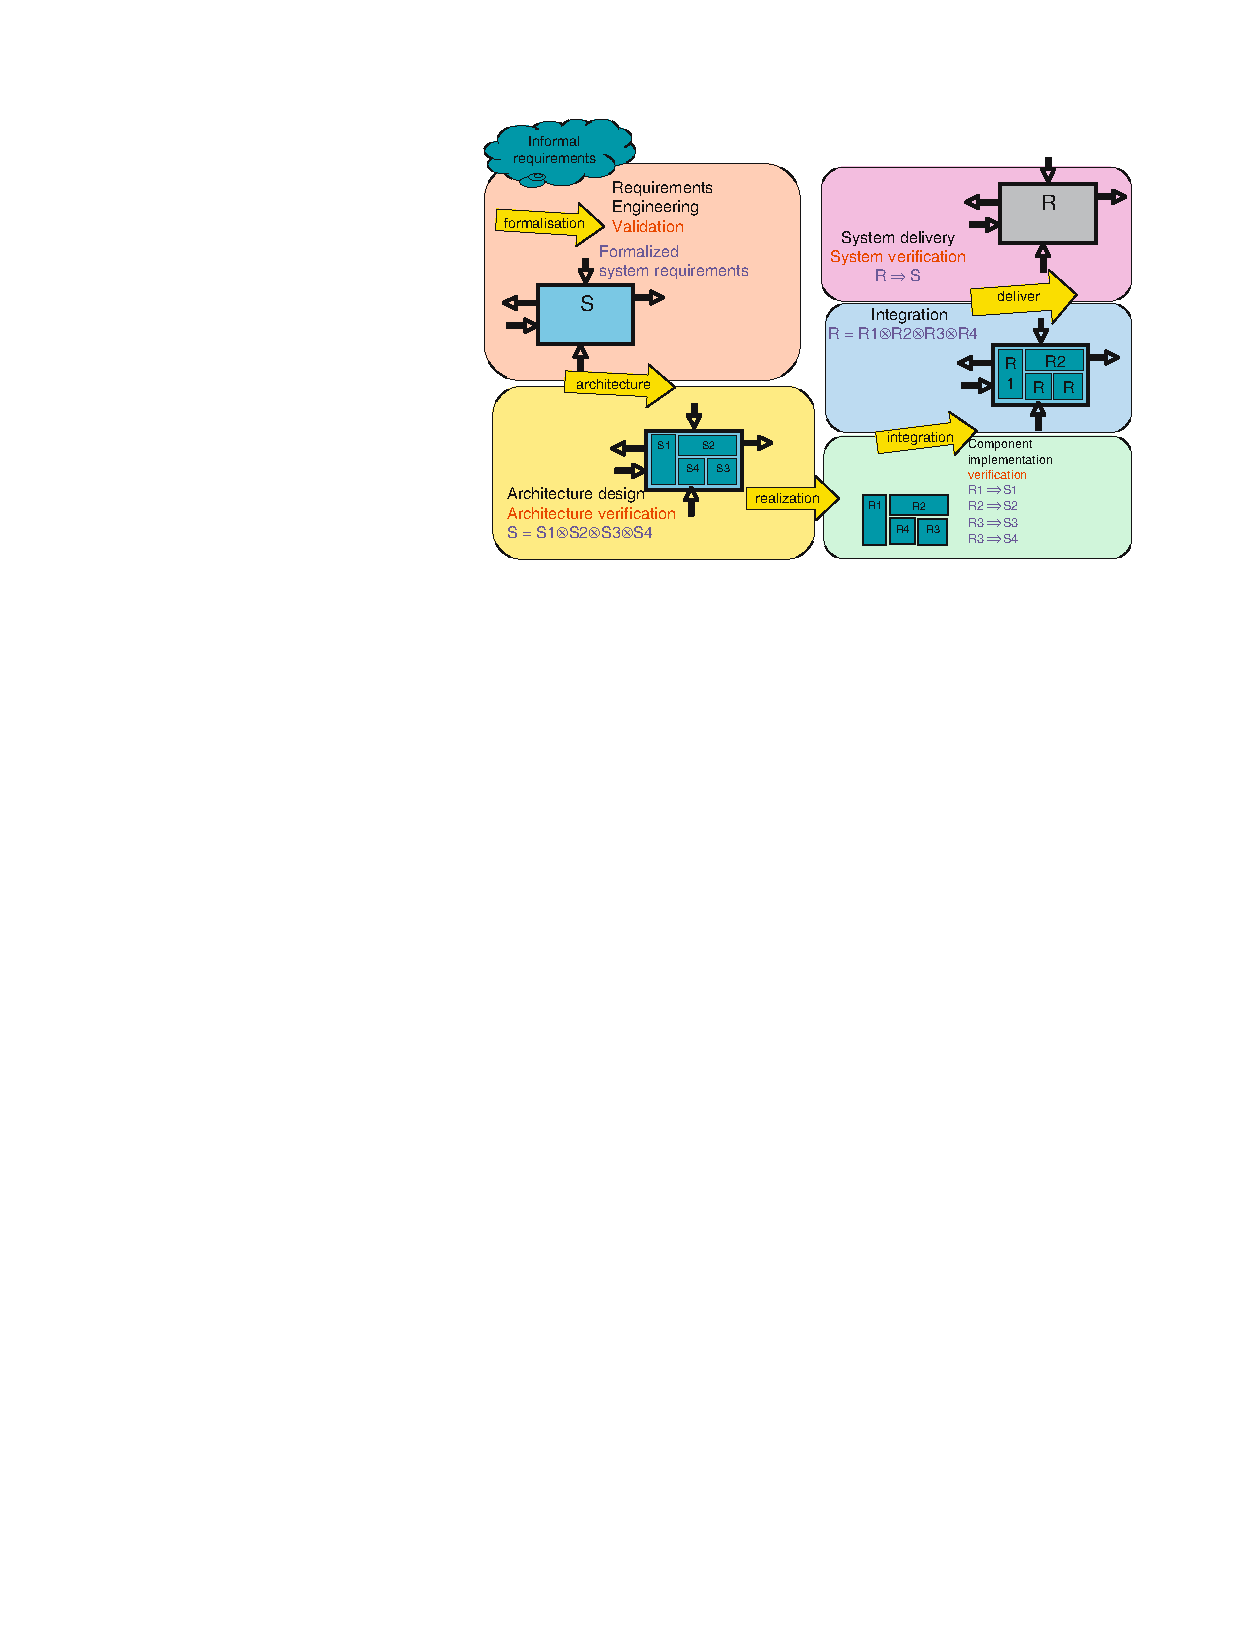
\includegraphics[width=9cm]{./images/MDE-broy.pdf}
   \end{center}
   \begin{flushright}
 (illustration from  [Broy, 2007])
   \end{flushright}
%   \end{block}
\end{slide}

\begin{slide}{Software Engineering}
So, ...  \dkb{yet another module in the MFES profile?}
\\

\begin{center}
   \fbox{Software architecture for reactive systems}
   \end{center}
~\\
~\\

\noindent
characterised by 
\begin{itemize}
\item \dgold{a methodological shift:} an \dkb{architectural} perspective
\item  \dgold{a focus:} on \dkb{reactive systems}
\end{itemize}
\end{slide}



\section{Software Architecture}


% \begin{slide}{What is software architecture?}
% \begin{block}{[Garlan \& Shaw, 1993]}
%  the systematic study of the overall structure of software systems
% \end{block}
% %\pause
% \begin{block}{[Perry \& Wolf, 1992]}
% SA = $\{$ Elements (\emph{what}), Form (\emph{how}), Rationale (\emph{why}) $\}$ 
% \end{block}
% %\pause
% \begin{block}{[Kruchten, 1995]}
%  deals with the design and implementation of the high-level structure of software
% \end{block}
% %\pause
% \begin{block}{[Britton, 2000]}
%  a discipline of generic design
% \end{block}
% \end{slide}
% \begin{slide}{What is software architecture?}
% \begin{block}{[Garlan \& Perry, 1995]}
%  the structure of the components of a program/system, their interrelationships, and principles and guidelines governing their design  and evolution over time
% \end{block}
% %\pause
% \begin{block}{[ANSI/IEEE Std 1471-2000]}
% the fundamental organisation of a system, embodied in its components, their relationships to each other and the environment, and the principles governing its design and evolution.
% \end{block}
% %\pause
% \begin{block}{[Garlan, 2003]}
%  a bridge between requirements and code (...) a blueprint for implementation.
% \end{block}
% \end{slide}

\begin{slide}{What is software architecture?}

The \dkb{architecture} of a system describes its gross structure which illuminates the top level design decisions, namely

\begin{itemize}
\item how is it \dgold{composed} and of which \dgold{interacting parts}?
\item where are the \dgold{pathways of interaction}?
\item which are the \dgold{key properties} of the parts the architecture rely and/or enforce?
\end{itemize}
\end{slide}


\begin{slide}{What is software architecture?}
A framework to perform early verification of a system and ensure composability of separately  developed parts, providing

\begin{itemize}
\item \dkb{structural} \emph{vs} \dkb{behavioural} views
\item \dkb{hierarchical} decomposition into interacting entities
\item \dkb{functional} \emph{vs} \dkb{non functional} properties
\\ (e.g. performance, reliability, dependability, portability, scalability, interoperability ...)
\\ to analyse schedulability, flow latency, memory consumption
\item \dkb{design guidelines} (e.g. binding threads to processors to make the system schedulable)
\item models for \dkb{adaptation} and \dkb{reconfigurability}
\item ...
\end{itemize}
\end{slide}



\begin{slide}{What is software architecture?}

\begin{block}{\fbox{Which structure? $\leadsto\;$ Architectural views}}
\begin{itemize}
\item \dkb{code-based structures}: such as \dkb{modules}, \dkb{classes}, \dkb{packages} and relationships like \dkb{uses}, \dkb{inherits from} or \dkb{depends on}.
\item \dkb{\underline{run-time structures}}: such as \dkb{object instances}, \dkb{clients}, \dkb{servers}, \dkb{databases},  \dkb{browsers}, \dkb{channels}, \dkb{broadcasters}, \dkb{software buses}, ...
\item \dkb{allocation structures}: intended to map code-based and run-time structures to external items, such as \dkb{network locations}, \dkb{physical devices}, \dkb{managerial structures} ...
\end{itemize}
\caixa{This course 
\begin{itemize}
\item  focus on \dkb{run-time structures} 
\item  and entails a particular \dkb{view}:  \dgold{components \& glue }
\end{itemize}
}
\end{block}
\end{slide}

\begin{slide}{What is software architecture?}
\begin{tabular}{@{}ll@{}}
\dkb{Components}: & 
\caixapeq[0.75]{
\dkb{\emph{Loci} of computation and data stores}, encapsulating subsets of the system's functionality and/or data;\\
Equipped with run-time interfaces defining their interaction points and restricting access to those subsets;\\
May explicitly define dependencies on their required execution contexts;\\
Typically provide \dkb{application-specific} services}\\
%\pause
\dkb{Connectors}: & 
\caixapeq[0.75]{Pathways of \dkb{interaction} between components;\\
Ensure the flow of data and regulates interaction;\\
Typically provide \dkb{application-independent} interaction facilities;\\
\dkb{\underline{Examples}}: procedure calls, pipes, wrappers, shared data structures, synchronisation barriers, etc.
}
\end{tabular}

\end{slide}

\begin{slide}{What is software architecture?}
\begin{tabular}{@{}ll@{}@{}}
\dkb{Configurations}: & 
\caixapeq{
Specifications of  \dkb{how} components and connectors \dkb{are associated};\\
\dkb{\underline{Examples}}: relations associating component \dkb{ports} to 
connector \dkb{roles}, mapping diagrams, etc.
}\\
%\pause
\dkb{Properties}: & 
\caixapeq{Set of \dkb{non functional} properties associated to any architectural element;\\
\dkb{\underline{Examples} (for components)}: availability, location, priority, CPU usage, ...\\
\dkb{\underline{Examples} (for connectors)}: reliability, latency, throughput, ...
}\\
\end{tabular}
\end{slide}

\begin{slide}{What is software architecture?}
\begin{tabular}{ll}
\dkb{Constraints}: & 
\caixapeq{
Represent claims about an architectural design that should remain true even as it evolves over time. Typical constraints include restrictions on allowable values of properties, topology, and design vocabulary. For example, \dgold{the number of clients of a particular server is less than some maximum value}.}\\
%\pause
\dkb{Styles}: & 
\caixapeq{Styles represent \dgold{families of related systems}. A style defines a vocabulary of design element types and rules for composing them.
 Examples include dataflow architectures based on  pipes and filters, blackboard architectures based on shared data space and a set of knowledge sources, and layered systems. 
}\\
%\pause
%\dkb{a metaphor}: & soccer vs water polo
\end{tabular}
\end{slide}


 

\begin{slide}{Two examples}
\fbox{from the \dkb{micro} level (a Unix shell script)}
~\\~\\~\\
\begin{center}
\texttt{cat invoices |  grep  january  | sort} 
\end{center}
~\\~\\
\begin{itemize}
\item
Application architecture can be understood based on very few rules
\item
Applications can be composed by non-programmers 
\item
... a simple architectural concept that can be comprehended and applied by a broad audience
\end{itemize}
\end{slide}



\begin{slide}{Two examples}
\fbox{to the \dkb{macro} level (the WWW architecture)}
~\\~\\
\begin{itemize}
\item
Architecture is totally  separated from the code
\item
There is no single piece of code that implements the architecture
\item
There are multiple pieces of code that implement the various components of the architecture
(e.g., different  browsers)
\item
One of the most successful applications is only understood adequately from an architectural  point of view
\end{itemize}
\end{slide}



\begin{slide}{Architectural styles (or patterns)}


An architectural style consists of:
\begin{itemize}
\item a set of \blue{component types} (e.g., process, procedure) that perform some function at runtime
\item  a topological \blue{layout} of the components showing their runtime relationships
\item a set of semantic \blue{constraints} (e.g. a layer may only talk to its adjacent)
\item a set of \blue{connectors} (e.g., data streams, sockets) that mediate communication among components
\end{itemize}
\end{slide}



\begin{slide}{Architectural styles (or patterns)}
\begin{itemize}
\item classify families of software architectures
\item act as \dkb{types} for \dkb{configurations}
\item provide
\begin{itemize}
\item \dkb{domain-specific design vocabulary} (eg, set of connector and component types admissible)
\item a set of \dkb{constraints} to single out which configurations are well-formed. Eg, a pipeline architecture might constraint valid configurations to be linear sequences of pipes and filters.
\item guidance for architectural design based on the \dkb{problem domain} and the \dkb{deployment context}
\end{itemize}
\end{itemize}
\end{slide}

\begin{slide}{Examples}
\begin{itemize}
\item \dkb{Layers}
\item \dkb{Client \& Server}
\item \dkb{Master \& Slave}
\item \dkb{Publish \& Subscribe}
\item \dkb{Peer2Peer}
\item \dkb{Pipes and Filters}
\item \dkb{Event-bus}
\item \dkb{Repositories}
\begin{itemize}
\item triggering by transactions: \dkb{databases}
\item triggering by current state: \dkb{blackboard}
\end{itemize}
\item \dkb{Table-driven} (virtual machines)
\item ...
\end{itemize}
\end{slide}


\begin{slide}{Pattern: Layers}
\begin{itemize}
\item helps to structure applications that can be decomposed into groups of subtasks at \dgold{different levels of abstraction}
\item Layer $n$ provides services to  layer $n+1$ implementing them through services of the layer $n+1$
\item Typically, service requests resort to synchronous procedure calls
\end{itemize}
~\\~\\
\begin{block}{Examples:}
\dkb{virtual machines} (eg, JVM)\\
\dkb{APIs} (eg, C standard library on top of Unix system calls)\\
\dkb{operating systems} (eg, Windows NT microkernel)\\
\dkb{networking protocols} (eg, ISO OSI 7-layer model; TCP/IP)
\end{block}
\end{slide}


\begin{slide}{Pattern: Client-Server}
\begin{itemize}
\item permanently active servers supporting multiple clients
\item requests typically handled in separate threads
\item stateless (session state maintained by the client) vs stateful servers
\item interaction by some inter-process communication mechanism
\end{itemize}
~\\~\\
\begin{block}{Examples:}
\dkb{remote DB access}\\
\dkb{web-based applications}\\
\dkb{interactive shells} 
\end{block}
\end{slide}

\begin{slide}{Pattern: Peer-2-Peer}
\begin{itemize}
\item symmetric Client-Service pattern
\item peers may change roles dynamically
\item services can be implicit (eg, through the use of a data stream)
\end{itemize}
~\\~\\
\begin{block}{Examples:}
\dkb{multi-user applications}\\
 \dkb{P2P file sharing} \\
\end{block}
\end{slide}



\begin{slide}{Pattern: Publish-Subscribe}
\begin{itemize}
\item used to structure distributed systems whose components interact through remote service invocations
\item servers publish their capabilities (services + characteristics) to a \dkb{broker} component, which accepts client requests and coordinate communication
\item allows dynamic reconfiguration
\item requires standardisation of service descriptions through IDL (eg CORBA IDL, .Net, WSDL) or
a binary standard (eg, Microsoft OLE --- methods are called indirectly using pointers)
\end{itemize}
~\\~\\
\begin{block}{Examples:}
\dkb{web services}\\
 \dkb{CORBA} (for cooperation among heterogeneous OO systems) \\
\end{block}
\end{slide}

\begin{slide}{Pattern: Master-Slave}
\begin{itemize}
\item a master component distributes work load to similar slave components and computes a final result from the results these slaves return
\item isolated slaves; no sharing of data
\item supports fault-tolerance and parallel computation
\end{itemize}
~\\~\\
\begin{block}{Examples:}
\dkb{dependable systems} 
\end{block}
\end{slide}

\begin{slide}{Pattern: Event-Bus}
\begin{itemize}
\item event sources publish messages to particular channels on an event bus
\item event listeners subscribe to particular channels  and are notified of message availability
\item asynchronous interaction
\item channels can be implicit (eg, using event patterns)
\item allows dynamic reconfiguration
\item variant of so-called \dkb{event-driven} architectures
\end{itemize}
~\\~\\
\begin{block}{Examples:}
\dkb{process monitoring} \\
\dkb{trading systems}
\end{block}
\end{slide}

\begin{slide}{Pattern: Pipe \& Filter}
\begin{itemize}
\item suitable for data stream processing
\item each processing step is encapsulated into a filter component
\item uniform data format
\item no shared state
\item concurrent processing is natural
\end{itemize}
~\\~\\
\begin{block}{Examples:}
\dkb{compilers} \\
\dkb{Unix shell commands}
\end{block}
\end{slide}

\begin{slide}{Pattern: Blackboard}
\begin{itemize}
\item suitable for problems with non deterministic solution strategy known
\item all components have access to a shared data store
\item components feed the blackboard and inspect it for new partial data
\item extending the data space is easy, but changing its structure may be hard
\end{itemize}
~\\~\\
\begin{block}{Examples:}
\dkb{complex IA problems} (eg, planning, machine learning) \\
\dkb{complex applications in computing science} (eg, speech recognition; computational chemistry)
\end{block}
\end{slide}


%\section{Evolution \& Challenges}
%

\begin{slide}{Software Architecture as a discipline}
\begin{itemize}
\item Until the 90's, SA was largely an \dkb{ad hoc affair} \\ (but see [Dijkstra,69], [Parnas79], ...)
\item Descriptions relied on informal box-and-line diagrams, rarely maintained once the system was built
\end{itemize}
\begin{block}{Challenges}
\begin{itemize}
\item recognition of a shared \dkb{repertoire} of methods, techniques and patterns for structuring complex systems
\item quest for \dkb{reusable frameworks} for the development of product families
\end{itemize}
\end{block}
\end{slide}

% \begin{slide}{The last 15 years}
% \begin{itemize}
% \item Formal notations for representing and analysing SA: \dkb{ADL}
% \item \dkb{Examples}: Wright, Rapide, SADL, Darwin, C2, Aesop, Piccola, AADL\\~\\
% \caixapeq{ADLs provide:
% \begin{itemize}
% \item \dkb{conceptual framework} + \dkb{concrete syntax}
% \item \dkb{tools} for parsing, displaying, analysing or simulating architectural descriptions
% \end{itemize}
% }\\~\\
% \item \textsc{Acme} [Garlan et al, 97] as an architectural \dkb{interchange} language (a sort of
% XML for architectural description)
% \item Use of model-based prototyping tools (eg Z, VDM) or model-checkers (eg Alloy) to 
% \dkb{analyse} architectural descriptions
% \end{itemize}
% \end{slide}


% \begin{slide}{The last 15 years}
% \begin{itemize}
% \item Classification of \dkb{architectural styles} characterising \dkb{families} of SA and acting as \dkb{types} for configurations
% \item \dkb{Standardisation} efforts: ANSI/IEEE Std 1471-2000, but also 'local' standards (eg, Sun's Enterprise JavaBeans architecture)
% \item Impact of the emergence of a \dkb{general purpose (object-oriented) design notation} --- UML ---
% closer to practitioners and with a direct link to OO implementations
% \item SA becomes a mature discipline in Software Engineering; new fields include \dkb{documentation} and  \dkb{architectural recovery} from legacy code
% \end{itemize}
% \end{slide}

\begin{slide}{Current trends}

\begin{block}{\rdb{Everyware everywhere}}
\begin{itemize}
\item \dkb{Everyware} products
\item vs \dkb{everywhere} development:\\ many companies look at themselves more as system \dkb{integrators} rather than as software \dkb{developers}:
~\\~\\
\caixapeq{
the code they write is \dkb{glue} code ...\\
which entails the need for common frameworks to reduce \dkb{architectural mismatchs} }
\end{itemize}
\end{block}
\end{slide}

\begin{slide}{Current trends}
\begin{block}{ From \rdb{object-oriented} to \rdb{component-based}}
\begin{center}
\caixa{\small
\begin{itemize}
\item In OO the architecture is \dkb{implicit}: source code exposes 
\dkb{class hierarchies} but not the \dkb{run-time interaction}
\item Objects are wired at a very low level and the description of the wiring patterns
is distributed among them
\item CBD retains the basic encapsulation of \dkb{data} and \dkb{code} principle to increase modularity
but shifts the emphasis from \dkb{class inheritance} to \dkb{object composition}
\item ... to avoid interference between inheritance and encapsulation
and pave the way to a development methodology based on \dkb{third-party assembly} of
components
\end{itemize}
}
\end{center}
\end{block}
\end{slide}


%\begin{slide}{Current trends}
%\begin{center}
%\fbox{CBD: the visual metaphor}
%\end{center}
%~\\~\\
%\begin{itemize}
%\item a  \dkb{palette} of computational units treated as \dkb{black boxes}
%\item and a  \dkb{canvas} into which they can be dropped
%\item \dkb{connections} are established by drawing \dkb{wires}
%\item which, typically, amounts to the invocation of some operation of the target component, given some
%suitable triggering condition on the source.
%\end{itemize}
%\end{slide}

\begin{slide}{Current trends}

\begin{block}{From \rdb{programming-in-the-large} to \rdb{ programming-in-the-world}}
\centering
~\\
\caixapeqq{
'not only the complexity of building a large application that one needs to deliver, in time and budget, to a client, but of managing an \dkb{open-ended
structure of autonomous components, possibly distributed and highly heterogeneous}.\\
This means developing software components that are autonomous and can be interconnected
with other components, software or otherwise, and \dkb{managing the interconnections
themselves} as new components may be required to join in and others to be
removed.'\\
\begin{flushright}
[Fiadeiro, 05]
\end{flushright}
}
\end{block}
\end{slide}

\section{The Course's Approach}
\begin{slide}{Challenges}
Such trends entails a number of challenges to the way we think about SA

\begin{itemize}
\item new \dkb{target}: need for an architectural discipline for \rdb{reactive systems}\\
(often \dkb{complex}, \dkb{time critical}, \dkb{mobile}, \dkb{cyber-physical}, etc ...) 
\item from  \dkb{composition}  to \rdb{coordination} (orchestration)
%\pause
\item relevance of \dkb{wrappers} and component \dkb{adapters}: integration \emph{vs} incompatible assumptions about component interaction
%~\\
%\caixapeq{
%'many resources cannot be smoothly integrated because they make incompatible assumptions about component interaction (...) Eg, it is hard to integrate a component packaged to interact via rpc, to
%another prepared to interact via shared data in  a proprietary trepresentation'\\
%(Garlan, 06)
%}
\item \dkb{reconfigurability}
\item  continued \rdb{interaction} as  a first-class citizen and the main form of software composition
\end{itemize}
\end{slide}



%----------------------------------------------------------------------------------
\begin{slide}{Reactive systems}
\small
\begin{block}{Reactive system}
\caixa{system that computes by reacting to stimuli from its environment along its overall computation}
\end{block}
\begin{itemize}
\item in contrast to sequential systems whose meaning is defined by the results of finite computations, the behaviour of reactive systems is mainly determined by \dkb{interaction} and \dkb{mobility} of \dkb{non-terminating} processes, 
evolving \dkb{concurrently}.
\item \dkb{observation} $\; \equiv\;$ interaction
\item \dkb{behaviour} $\; \equiv\;$ a structured record of interactions
\end{itemize}
\end{slide}

%----------------------------------------------------------------------------------
\begin{slide}{Reactive systems}
\small
\begin{block}{Concurrency vs interaction}
\begin{align*}
& \mathsf{x : = 0;}\\
& \mathsf{x := x+1\mid x := x+2}
\end{align*}
\end{block}
\begin{itemize}
\item both statements in \dgold{parallel} could read $x$ before it is written 
\item which values can $x$ take?
\item which is the program outcome if \dgold{exclusive access} to memory and \dgold{atomic execution}
of assignments is guaranteed?
\end{itemize}
\end{slide}



%\begin{slide}{}
%\begin{itemize}
%\item What is Software Architecture?
%%\item    Architectural Styles
%\item Evolution \& Challenges
%\item \dkb{Course perspective: Architecture for Reactive Systems}
%\end{itemize}
%\end{slide}



%\begin{slide}{Starting point}
%SA as studied at \dkb{MFES (until now)}: 
%\begin{center}
%\fbox{the architecture of \dkb{functional designs}}
%\end{center} ~\\~\\
%\begin{tabular}{ll}
%\dkb{Interfaces}: & $f :: \cdots \longrightarrow \cdots$\\
%\dkb{Components}: & $f = \cdots$\\
%\dkb{Connectors}: &  $�$, $\split{~}{~}$, $\times$, $+$, ...\\
%\dkb{Configurations}: &  functions assembled by composition\\
%\dkb{Properties}: & invariants (pre-, post-conditions)\\
%\dkb{Behavioural effects}: & monads and Kleisli compostion\\
%\dkb{Underlying maths}: & universal algebra and relational calculus\\
%\end{tabular}
%\end{slide}

%\begin{slide}{The challenge}
%Software Architecture is  challenged by the continuous evolution towards very large, heterogeneous, highly dynamic computing systems, whose behaviour  cannot be  characterized in terms of a io-relation In most cases, such a behaviour
%\begin{itemize}
%\item is potentially \dkb{non-terminating}, 
%\item  expresses a \dkb{continued interaction} with the system's environment and sub-systems which execute
%\dkb{concurrently} in distributed, often loosely coupled configurations.
%\end{itemize}
%\end{slide}

\begin{slide}{Our approach}
\begin{center}
\caixa{
There is no \dkb{general-purpose, universally tailored}, approach to  architectural design of \dkb{complex} and \dkb{reactive} systems
}
\end{center}
~\\

%\pause
Therefore, the course
\begin{itemize}
\item introduces different models for \dkb{reactive} systems
\item discusses their \dkb{architectural design} and \dkb{analysis}
\item with (reasonable) \dkb{tool support}  for modelling and analysis 
\end{itemize}
\end{slide}

\begin{slide}{Syllabus} 
\begin{itemize}
\item Introduction to software architecture
\item \rdb{Background}
\begin{itemize}
\item \dkb{Introduction to transition systems} 
  (\dgold{\textsf{mCRL2}})
\item \dkb{Introduction to modal, hybrid and dynamic logic}
  (\dgold{\textsf{mCRL2}})
\end{itemize}
\item \rdb{Models and calculi of reactive systems}
\begin{itemize}
%\item \dkb{Classical (non deterministic)}  (\dgold{\textsf{mCRL2}})
\item \dkb{Timed (with real time constraints)} (\dgold{\textsf{Uppaal}})
%\item \dkb{Probabilistic}  (\dgold{\textsf{PRISM}})
%\item \dkb{Cyber-physical} (\dgold{\textsf{KeYmaera}})
% \item \transp[30]{Probabilistic  ({\textsf{PRISM}})}
% \item \transp[30]{{Cyber-physical} ({\textsf{KeYmaera}})}
\end{itemize}
\item \rdb{Architecture for reactive systems}
\begin{itemize}
%\item \dkb{An architectural description language} (\dgold{\textsf{AADL}})
\item \dkb{Component-oriented architectural design}
\begin{itemize}
\item  \dkb{Paradigm:} Software components as monadic Mealy machines
%\item \dkb{Foundations:}  Coalgebra theory as a semantic framework for state-based systems a component calculus
\item \dkb{Method:} The \dgold{\textsf{mMm}} calculus; prototyping in  \dgold{\textsc{Haskell}}
\end{itemize}
\item  \dkb{Coordination-oriented architectural design}
\begin{itemize}
\item  \dkb{Paradigm:} The  \dgold{\textsf{Reo}} exogenous coordination model
\item \dkb{Method:} Compositional specification of the glue layer 
\end{itemize}
\end{itemize}
\end{itemize}
\end{slide}




%\begin{slide}{Component-oriented architectural design}
%\fbox{components \& ports (the Stack diagram in a component calculus)}
%~\\~\\
%\scriptsize
%\begin{align*}
%\begin{cases}
%\fuc{pop} : & \SING \longrightarrow E \\
%\fuc{top} : & \SING \longrightarrow E \\
%\fuc{push} : & E \longrightarrow  \SING
%\end{cases}
%& \qquad \qquad
%\xygraph{~{<2pc,0pc>:} []!{
%      +0="q1" *=<-10pt>{ }
%      ; p!D**{},
%       ; "q1"  -/-20pt/*{} +0
%       ;p-/:a(90)80pt/="X11"**\dir{-}
%       ; ?(.3)="ka1",
%       p-/:a(90)36pt/**\dir{-}="X22"
%       ;p-/:a(90)80pt/="X33"**\dir{-}
%       ; ?(.3)="ja1",
%       p-/:a(90)36pt/**\dir{-}
%       ; "ja1"  *{\bullet} +0
%       ; "ka1" -/2pt/*!E\cir<2pt>{} +0
%       ; <-13pt,17pt>+"ja1" *{\fuc{Stack}} +0
%       ; "ka1"}
%("ja1"[d]{E + E + \SING \; \; \rdb{=}\; \; \dkb{O}}
%- "ja1" "ka1"[u]{\SING+\SING+E \; \; \rdb{=}\; \; \dkb{I}} - "ka1" )}
%\end{align*}
%\end{slide}


% \begin{slide}{Component-oriented architectural design}
% ~\\
% \fbox{new components from old in \textsc{mMm}}
% ~\\

% \scriptsize

% \begin{equation*}
% \xygraph{~{<2pc,0pc>:} []!{
%       +0="q1" *=<10pt>{ }
%      ; p!D**{},
%       ; "q1"  -/0pt/*{} +0
%       ;p-/:a(90)150pt/="X11"**\dir{-}
%       ; ?(.3)="ka1",
%       p-/:a(90)36pt/**\dir{-}="X22"
%       ;p-/:a(90)150pt/="X33"**\dir{-}
%       ; ?(.3)="ja1",
%       p-/:a(90)36pt/**\dir{-}
%       ; "ja1"  *{\bullet} +0
%       ; <0pt,10pt>+"ja1"  +0
% %       ; <0pt,10pt>+"ja1" *{\dois^{{4}^{n}}} +0
%       ; "ka1" -/2pt/*!E\cir<2pt>{} +0
%       ; <-15pt,-20pt>+"ka1" *{\dois^n} +0
%       ; <30pt,-17pt>+"ja1" *{\fuc{Cell} \para \fuc{Cell} \para \cdots \para \fuc{Cell}} +0
%      ; "ka1"
%       , "q1"."ja1"."ka1"."X11"."X22"."X33"}="C"
%   ( "ja1"[uu]{\dois^{{4}^{n}}} - "ja1"   "ja1"[u]="lkg1" "ja1"[urr]="lkg4")
%  "C"[d(3)]!{
%      +0="q2" *=<10pt>{ }
%      ; p!D**{},
%       ; "q2"  -/0pt/*{} +0
%       ;p-/:a(90)60pt/="X11"**\dir{-}
%       ; ?(.3)="ka2",
%       ?(.7)="kb2",
%       p-/:a(90)36pt/**\dir{-}="X22"
%       ;p-/:a(90)60pt/="X33"**\dir{-}
%       ; ?(.26)="ja2",
%       ?(.7)="jb2",
%       p-/:a(90)36pt/**\dir{-}
%       ; "ja2" *{\bullet} +0
%      ; "ka2"  -/2pt/*!E\cir<2pt>{} +0
%       ; <13pt,-17pt>+"ja2" *{\fuc{Bus}} +0
%       , "q2"."ja2"."ka2"."X11"."X22"."X33"}
%   ( "ja2" "ka2"[dd]{\dois^{{4}^{n}}} - "ka2" "ja2"[u]="lig2" "ka2"[d]="lkg2" )
%  "ka1" - "ja2"
%  "lkg2" - [r</8ex/] - [u!{"lkg1";p+/r/}] - [l</8ex/] -  "lkg1" - [r</3ex/] }
% \end{equation*}
% ~\\

% \begin{align*}
% \fuc{GameLife} \;& =\; \feed{((\fuc{Cell} \para \fuc{Cell} \para \cdots \para \fuc{Cell}) \qcomp \fuc{Bus})}\\
% \intertext{where}
% \fuc{Bus} \;& =\; \flift{\fuc{w}}
% \end{align*}

% \end{slide}





% %\begin{slide}{Process-oriented architectural design}
% %\fbox{a configuration (client-server in \textsc{Acme})}
% %~\\~\\
% %~\\
% %
% %\texttt{
% %System CS = $\{$\\ 
% %\hspace{0.5cm} \underline{component} client = $\{$ \underline{port} call $\}$\\
% %\hspace{0.5cm} \underline{component} server = $\{$ \underline{port} request $\}$\\
% %\hspace{1cm} \underline{property} max-clients-supported = 10;\\
% %\hspace{0.5cm} \underline{connector} rpc = $\{$ \underline{role} plug-cl;   \underline{role} plug-sv$\}$\\
% %\hspace{0.5cm} $\}$\\
% %\hspace{0.5cm} \underline{attachments} = $\{$\\ 
% %\hspace{1cm} $\{$ call  \underline{to} plug-cl ; server  \underline{to} plug-sv $\}$\\
% %\hspace{0.5cm} $\}$
% %}
% %\end{slide}
% %



% \begin{slide}{Coordination-oriented architectural design}
% \fbox{a connector (synchronization barrier) in \textsc{Reo}}
% ~\\~\\

% \begin{displaymath}
%     \xymatrix@R=1em@C=2em{ & & \bullet\; \ar@{-{>}}[r]^{\sync} &\; c\\
%               a\; \ar@{-{}}[r] & \bullet \ar@/^/[ur] \ar@/_/[dr] & &\\
%                & & \bullet\; \ar@{|-{|}}[d] &\; \\
%                & & \bullet\; &\\
%               b\; \ar@{-{}}[r] & \bullet \ar@/^/[ur] \ar@/_/[dr] & &\\
%               & & \bullet\; \ar@{-{>}}[r]^{\sync} &\; d\\
%               }
% \end{displaymath}
% \end{slide}


%\begin{slide}{Our approach}
%\begin{itemize}
%\item \dkb{Time-critical systems}, i.e., systems whose design correctness is assessed not only in terms of the logical result of computation but also depends on the time at which such results are produced.
%\pause
%\item \dkb{Service-oriented applications}.  Services are dynamic entities, running on different platforms often owned by different organisations, interacting through public interfaces, and typically remaining loosely coupled, if not utterly unaware of each other. Open, dynamic reconfigurable and evolutive structure.
%\end{itemize}
%\end{slide}
%
%\begin{slide}{Our approach}
%\begin{center}
%\caixapeq{\rdb{+} a module on \dkb{performance and dependability analysis in software architecture}}
%\end{center}
%~\\
%\begin{itemize}
%\item to model \dkb{unreliable behaviour}
%\item  to forecast system \dkb{performance and dependability}
% \end{itemize}
%\end{slide}



%
%
%
%\item (\underline{semantics})  Timed utomata and their calculus
%\item (\underline{logic})  Behavioural properties with time-constraints 
%\item (\underline{tool support})  \textsc{mCRL2} and \textsc{Uppaal}
%\end{itemize}
%\end{itemize}
%%\item (\underline{foundations}) Algebraic structure \emph{vs} coalgebraic behaviour
%\item (\underline{modeling}) Process algebra 
%\item (\underline{logic}) Expressing and verifying behavioural properties
%\item (\underline{tool support}) \textsc{mCRL2}
%
%\end{slide}
%
%\begin{slide}{Syllabus} 
%\begin{itemize}
%\item (\emph{Case-study 2}) \rdb{Service-oriented architectures}
%\begin{itemize}
%\item (\underline{characterisation}) Problems and examples
%\item (\underline{semantics})  Exogenous coordination models
%\item (\underline{method \& tool support})   \textsc{Orc} \\(\dgold{asynchronous, dynamic coordination language})
%\item (\underline{method \& tool support})   \textsc{Reo}\\ (\dgold{connector-based coordination language})
%\end{itemize}
%\item  \rdb{Performance and dependability in software architecture}
%\begin{itemize}
%\item (\underline{modelling}) Stochastic behaviour, dependability and performance evaluation
%\item (\underline{foundations}) Markov chains and markovean decision processes
%\item (\underline{tool support}) \textsc{Prism}
%\end{itemize}
%\end{itemize}
%\end{slide}


\begin{slide}{Pragmatics ...} 
\begin{itemize}
%\item \textbf{References:} (tba)
\item \textbf{Assessment:} 
\begin{itemize}
\item \dkb{Test}  \dkb{in June} - 60 \% \\
%\item \dkb{Special Lab Assessment} (for \dkb{Models for cyber-physical systems}, \dkb{28 March}) - 20 \%
\item \dkb{Group projects (3x)}  - 40 \%~~(10+15+15)
\end{itemize}
~\\
%\item{Website:}
%\begin{itemize}
%  \item \url{http://ac1516.proenca.org}
%\end{itemize}
\myblock{\dkb{\url{http://wiki.di.uminho.pt/twiki/bin/view/Education/MFES/AC}}\\[3mm]
{\small \url{http://ac1617.proenca.org} }}
% \myblock{\dkb{\url{http://ac1617.proenca.org}}}
~\\
%\item \textbf{... may be extended} (with reasonable limits) by contacting \texttt{lsb@di.uminho.pt}
\item \textbf{Research context:} Projects 
\begin{itemize}
%\item \textsc{Mondrian}  --- 2011-13 
%\\ on \dgold{foundations for architectural design}
% \item 
% \textsc{Nasoni}  --- 2012-15
% \\ on \dgold{heterogenous software coordination
% \\ (continuous vs discrete systems)}
\item
\textsc{Dali}  --- 2016-18
\\ on \dgold{Dynamic logics for cyber-physical systems}
\item
\textsc{Trust}  --- 2016-18
\\ on \dgold{Trustworthy Software Design with Alloy}
\end{itemize}

\end{itemize}

\begin{center}
\rdb{possible GRANTS available! } \\ 
(with U. Nijmegen, U. Aveiro, CWI, INESC TEC)
\end{center}
\end{slide}






%
%\begin{slide}{To be extended to }
%\begin{itemize}
%\item \dkb{object}-based designs: attribute-method interfaces; interaction by method calling
%\pause
%\item \dkb{process}-based designs: interfaces are \dkb{sets of actions} whose transformational meaning is largely ignored; richer composition mechanisms; interaction by \dkb{action handshake}.
%\pause 
%\item \dkb{service}-based designs: interfaces as  \dkb{sets of ports} through which data flows; interaction is \dkb{anonymous} and handled by complex \dkb{connectors}; clear separation between \dkb{computation} and \dkb{coordination}
%\end{itemize}
%\end{slide}

%

%\begin{slide}{To be extended to }
%\begin{tabular}{l|lll}
%\begin{tabular}{c}
%Paradigm \\ vs\\
%Orchestration
%\end{tabular}
%&  \dkb{Objects} &  \dkb{Processes} &  \dkb{Services} \\ \hline\\
% \dkb{Endogenous} &  mMm & \textsc{Ccs}, $\pi$ & \\
% \dkb{Exogenous} &  & \textsc{Orc} &\textsc{Reo}\\
% \hline\\
%\end{tabular}
%~\\~\\~\\
%where\\
%\noindent
%\textsc{Ccs}, $\pi$-\emph{calculus} (Milner,80) and (Milner, 92)\\
%\textsc{Reo} (Arbab, 03)\\
%\textsc{Orc} (Misra et al, 02)\\
%mMm: monadic Mealy machines (Barbosa \& Oliveira, 01)\\
%\end{slide}

%
%\begin{slide}{Semantics}
%We need a mathematical semantics able to take into account
%\begin{itemize}
%\item \dkb{persistence}, i.e., internal state and state transitions
%\item \dkb{continued interaction} along the whole computational process
%\item \dkb{ potential infinite behaviour}
%\item  equational and inequational reasoning in terms of  \dkb{observational} preorders
%\end{itemize}
%\pause
%These requirements lead to \dkb{coalgebra theory} (Rutten, 96)  as \\
%\begin{center}
%\fbox{the mathematics of state-based systems}
%\end{center}
%\end{slide}

%\begin{slide}{Syllabus}
%\begin{enumerate}
%\item Introduction to Software Architecture
%\item Foundations: coalgebra and coinduction
%\item Process-oriented architectures (\textsc{Ccs}, $\pi$-\emph{calculus},\textsc{Orc})
%\item Service-oriented architectures (\textsc{Reo}) 
%\item Object-oriented architectures (monadic Mealy machines)
%\end{enumerate}
%\end{slide}

%\begin{slide}{Exercise}
%Read, discuss, comment \& present to the class one of the following papers
%\begin{enumerate}
%\item \dkb{Architecture-driven modelling and analysis}, D. Garlan and B. Schmerl, SCS'06, 2006.
%\item \dkb{Analysing architectural styles with Alloy}, J. S. Kim and D. Garlan, ROSATEA'06, 2006.
%\item \dkb{Modelling software architectures in the UML}, N. Medvidovic, D. Rosenblum, D. Remiles, and J. Robbins, \emph{ACM Trans. on Software Engineering and Methodology}, 11(1), 2002.
%\item \dkb{Software services: Scientific challenge or industrial hype?}, J. L. Fiadeiro, TAC
%LNCS 3407, Springer, pp. 1-13, 2005.
%\item \dkb{ArchJava: Connecting software architecture to implementation}, J. Aldrich, C. Chambers, and D. Notkin.
%\end{enumerate}
%\end{slide}

%
\end{document}
